\documentclass[]{article}
\usepackage{lmodern}
\usepackage{amssymb,amsmath}
\usepackage{ifxetex,ifluatex}
\usepackage{fixltx2e} % provides \textsubscript
\ifnum 0\ifxetex 1\fi\ifluatex 1\fi=0 % if pdftex
  \usepackage[T1]{fontenc}
  \usepackage[utf8]{inputenc}
\else % if luatex or xelatex
  \ifxetex
    \usepackage{mathspec}
  \else
    \usepackage{fontspec}
  \fi
  \defaultfontfeatures{Ligatures=TeX,Scale=MatchLowercase}
\fi
% use upquote if available, for straight quotes in verbatim environments
\IfFileExists{upquote.sty}{\usepackage{upquote}}{}
% use microtype if available
\IfFileExists{microtype.sty}{%
\usepackage{microtype}
\UseMicrotypeSet[protrusion]{basicmath} % disable protrusion for tt fonts
}{}
\usepackage[margin=1in]{geometry}
\usepackage{hyperref}
\hypersetup{unicode=true,
            pdfborder={0 0 0},
            breaklinks=true}
\urlstyle{same}  % don't use monospace font for urls
\usepackage{graphicx,grffile}
\makeatletter
\def\maxwidth{\ifdim\Gin@nat@width>\linewidth\linewidth\else\Gin@nat@width\fi}
\def\maxheight{\ifdim\Gin@nat@height>\textheight\textheight\else\Gin@nat@height\fi}
\makeatother
% Scale images if necessary, so that they will not overflow the page
% margins by default, and it is still possible to overwrite the defaults
% using explicit options in \includegraphics[width, height, ...]{}
\setkeys{Gin}{width=\maxwidth,height=\maxheight,keepaspectratio}
\IfFileExists{parskip.sty}{%
\usepackage{parskip}
}{% else
\setlength{\parindent}{0pt}
\setlength{\parskip}{6pt plus 2pt minus 1pt}
}
\setlength{\emergencystretch}{3em}  % prevent overfull lines
\providecommand{\tightlist}{%
  \setlength{\itemsep}{0pt}\setlength{\parskip}{0pt}}
\setcounter{secnumdepth}{0}
% Redefines (sub)paragraphs to behave more like sections
\ifx\paragraph\undefined\else
\let\oldparagraph\paragraph
\renewcommand{\paragraph}[1]{\oldparagraph{#1}\mbox{}}
\fi
\ifx\subparagraph\undefined\else
\let\oldsubparagraph\subparagraph
\renewcommand{\subparagraph}[1]{\oldsubparagraph{#1}\mbox{}}
\fi

%%% Use protect on footnotes to avoid problems with footnotes in titles
\let\rmarkdownfootnote\footnote%
\def\footnote{\protect\rmarkdownfootnote}

%%% Change title format to be more compact
\usepackage{titling}

% Create subtitle command for use in maketitle
\newcommand{\subtitle}[1]{
  \posttitle{
    \begin{center}\large#1\end{center}
    }
}

\setlength{\droptitle}{-2em}
  \title{}
  \pretitle{\vspace{\droptitle}}
  \posttitle{}
  \author{}
  \preauthor{}\postauthor{}
  \date{}
  \predate{}\postdate{}


\begin{document}

\section{Red Wine Quality by Hammad
Al-Hammad}\label{red-wine-quality-by-hammad-al-hammad}

\begin{quote}
\textbf{What is the Red Wine?}: Red wine is a type of wine made from
dark-colored (black) grape varieties. The actual color of the wine can
range from intense violet, typical of young wines, through to brick red
for mature wines and brown for older red wines. The juice from most
purple grapes is greenish-white; the red color comes from anthocyan
pigments (also called anthocyanins) present in the skin of the grape;
exceptions are the relatively uncommon teinturier varieties, which
produce a red colored. Much of the red-wine production process therefore
involves extraction of color and flavor components from the grape skin.
\end{quote}

\begin{quote}
\textbf{What is the dataset?}: This tidy data set contains 1,599 red
wines with 11 variables on the chemical properties of the wine. At least
3 wine experts rated the quality of each wine, providing a rating
between 0 (very bad) and 10 (very excellent).
\end{quote}

\begin{quote}
\textbf{Data Overview:} This dataset is public available for research.
The details are described in {[}Cortez et al., 2009{]}.
\end{quote}

Input variables (based on physicochemical tests):

1 - fixed acidity (tartaric acid - g / dm\^{}3)

2 - volatile acidity (acetic acid - g / dm\^{}3)

3 - citric acid (g / dm\^{}3)

4 - residual sugar (g / dm\^{}3)

5 - chlorides (sodium chloride - g / dm\^{}3

6 - free sulfur dioxide (mg / dm\^{}3)

7 - total sulfur dioxide (mg / dm\^{}3)

8 - density (g / cm\^{}3)

9 - pH

10 - sulphates (potassium sulphate - g / dm3)

11 - alcohol (\% by volume)

12 - quality (score between 0 and 10)

\paragraph{Now, We are going to load data into the workspace.Then, we
are going to print the internal structure of the
dataset.}\label{now-we-are-going-to-load-data-into-the-workspace.then-we-are-going-to-print-the-internal-structure-of-the-dataset.}

\begin{verbatim}
## 'data.frame':    1599 obs. of  13 variables:
##  $ X                   : int  1 2 3 4 5 6 7 8 9 10 ...
##  $ fixed.acidity       : num  7.4 7.8 7.8 11.2 7.4 7.4 7.9 7.3 7.8 7.5 ...
##  $ volatile.acidity    : num  0.7 0.88 0.76 0.28 0.7 0.66 0.6 0.65 0.58 0.5 ...
##  $ citric.acid         : num  0 0 0.04 0.56 0 0 0.06 0 0.02 0.36 ...
##  $ residual.sugar      : num  1.9 2.6 2.3 1.9 1.9 1.8 1.6 1.2 2 6.1 ...
##  $ chlorides           : num  0.076 0.098 0.092 0.075 0.076 0.075 0.069 0.065 0.073 0.071 ...
##  $ free.sulfur.dioxide : num  11 25 15 17 11 13 15 15 9 17 ...
##  $ total.sulfur.dioxide: num  34 67 54 60 34 40 59 21 18 102 ...
##  $ density             : num  0.998 0.997 0.997 0.998 0.998 ...
##  $ pH                  : num  3.51 3.2 3.26 3.16 3.51 3.51 3.3 3.39 3.36 3.35 ...
##  $ sulphates           : num  0.56 0.68 0.65 0.58 0.56 0.56 0.46 0.47 0.57 0.8 ...
##  $ alcohol             : num  9.4 9.8 9.8 9.8 9.4 9.4 9.4 10 9.5 10.5 ...
##  $ quality             : int  5 5 5 6 5 5 5 7 7 5 ...
\end{verbatim}

As listed above, the data contains 1599 obs. of 13 variables. The first
variable (X) is useles in our analysis. So, we are going to delete it.

\paragraph{Experts in alcohol always categorize them to 3 types of
effectiveness:}\label{experts-in-alcohol-always-categorize-them-to-3-types-of-effectiveness}

\begin{enumerate}
\def\labelenumi{\arabic{enumi}.}
\item
  Light: Alcohol \textless{} 9
\item
  Medium: Alcohol \textgreater{}= 9 and Alcohol \textless{}= 12
\item
  Strong: Alcohol \textgreater{} 12
\end{enumerate}

\emph{So, We are going to add new column to categorize the wine type if
it's Light, Medium or Strong.}

\paragraph{Let's see how many one of our sample in each
category.}\label{lets-see-how-many-one-of-our-sample-in-each-category.}

\begin{verbatim}
## 
##  Light Medium Strong 
##     37   1421    141
\end{verbatim}

As we see, Light = 37, Medium = 1421 and Strong = 141

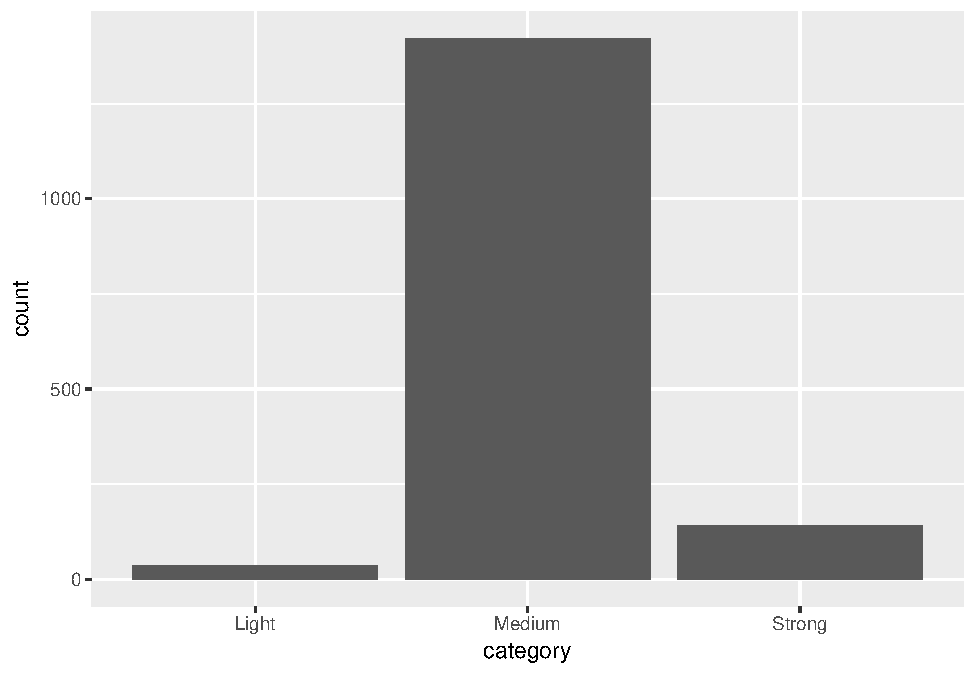
\includegraphics{RedWine_files/figure-latex/Disiplay_QPlot_Category-1.pdf}

\paragraph{Experts in alcohol also ranking them to 3 types of
quality:}\label{experts-in-alcohol-also-ranking-them-to-3-types-of-quality}

\begin{enumerate}
\def\labelenumi{\arabic{enumi}.}
\item
  Poor: Quality \textless{} 9
\item
  Good: Quality \textgreater{}= 9 and Quality \textless{}= 12
\item
  Excellent: Quality \textgreater{} 12
\end{enumerate}

\emph{So, We are going to add new column to rank the wine type if it's
Poor, Good or Excellent}

\paragraph{Let's see how many one of our sample in each
ranking}\label{lets-see-how-many-one-of-our-sample-in-each-ranking}

\begin{verbatim}
## 
## Excellent      Good      Poor 
##        18       837       744
\end{verbatim}

As we see, Excellent = 18, Good = 837 and Poor = 744

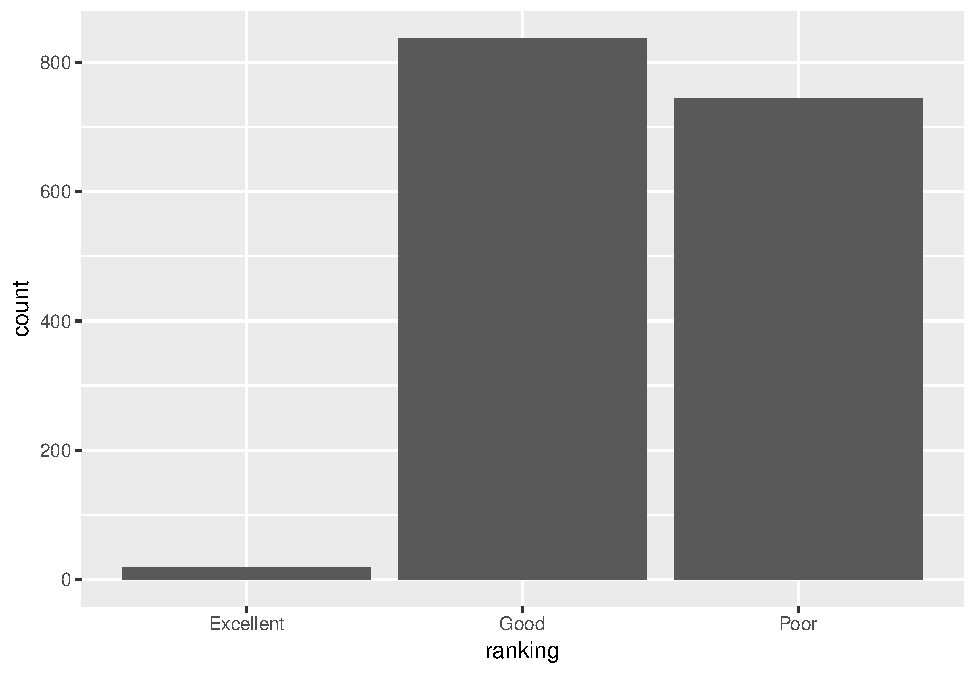
\includegraphics{RedWine_files/figure-latex/Disiplay_QPlot_Ranking-1.pdf}

\section{Univariate Plots Section}\label{univariate-plots-section}

\begin{quote}
\textbf{Tip}: Here, we are going to perform some preliminary exploration
of Red Wines dataset.
\end{quote}

\begin{verbatim}
##  fixed.acidity   volatile.acidity  citric.acid    residual.sugar  
##  Min.   : 4.60   Min.   :0.1200   Min.   :0.000   Min.   : 0.900  
##  1st Qu.: 7.10   1st Qu.:0.3900   1st Qu.:0.090   1st Qu.: 1.900  
##  Median : 7.90   Median :0.5200   Median :0.260   Median : 2.200  
##  Mean   : 8.32   Mean   :0.5278   Mean   :0.271   Mean   : 2.539  
##  3rd Qu.: 9.20   3rd Qu.:0.6400   3rd Qu.:0.420   3rd Qu.: 2.600  
##  Max.   :15.90   Max.   :1.5800   Max.   :1.000   Max.   :15.500  
##    chlorides       free.sulfur.dioxide total.sulfur.dioxide
##  Min.   :0.01200   Min.   : 1.00       Min.   :  6.00      
##  1st Qu.:0.07000   1st Qu.: 7.00       1st Qu.: 22.00      
##  Median :0.07900   Median :14.00       Median : 38.00      
##  Mean   :0.08747   Mean   :15.87       Mean   : 46.47      
##  3rd Qu.:0.09000   3rd Qu.:21.00       3rd Qu.: 62.00      
##  Max.   :0.61100   Max.   :72.00       Max.   :289.00      
##     density             pH          sulphates         alcohol     
##  Min.   :0.9901   Min.   :2.740   Min.   :0.3300   Min.   : 8.40  
##  1st Qu.:0.9956   1st Qu.:3.210   1st Qu.:0.5500   1st Qu.: 9.50  
##  Median :0.9968   Median :3.310   Median :0.6200   Median :10.20  
##  Mean   :0.9967   Mean   :3.311   Mean   :0.6581   Mean   :10.42  
##  3rd Qu.:0.9978   3rd Qu.:3.400   3rd Qu.:0.7300   3rd Qu.:11.10  
##  Max.   :1.0037   Max.   :4.010   Max.   :2.0000   Max.   :14.90  
##     quality        category         ranking   
##  Min.   :3.000   Light :  37   Excellent: 18  
##  1st Qu.:5.000   Medium:1421   Good     :837  
##  Median :6.000   Strong: 141   Poor     :744  
##  Mean   :5.636                                
##  3rd Qu.:6.000                                
##  Max.   :8.000
\end{verbatim}

The result above is listing basic statistics about each variable.

\paragraph{Here is a histogram about the fixed.acidity
variable.}\label{here-is-a-histogram-about-the-fixed.acidity-variable.}

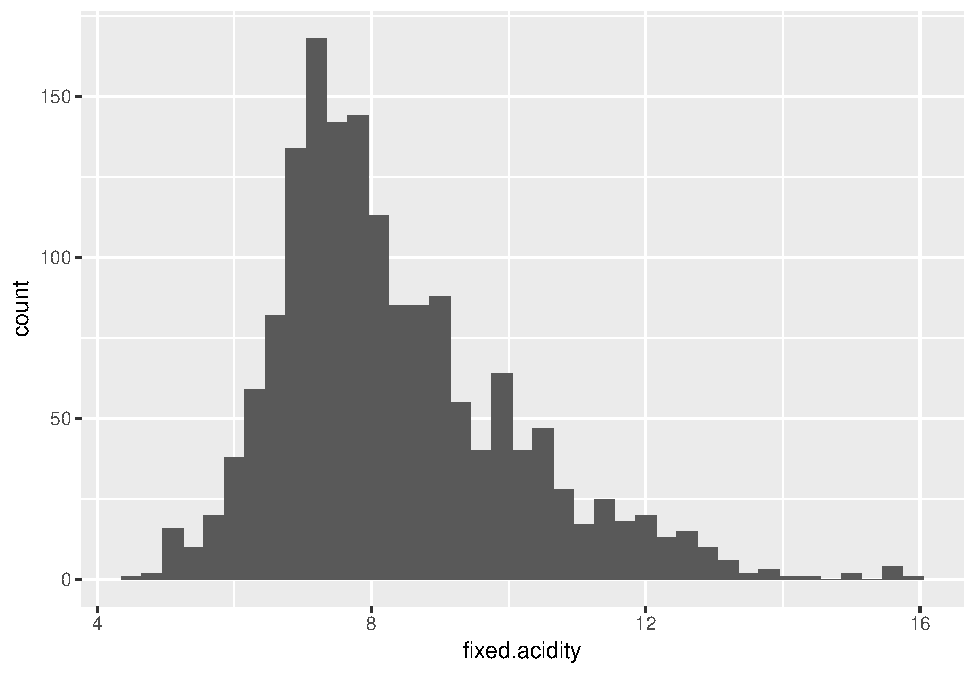
\includegraphics{RedWine_files/figure-latex/Make_Plot_Function_For_fixed.acidity-1.pdf}

The fixed.acidity is skewed to the right.

\paragraph{Here is a summary about the fixed.acidity
variable.}\label{here-is-a-summary-about-the-fixed.acidity-variable.}

\begin{verbatim}
##    Min. 1st Qu.  Median    Mean 3rd Qu.    Max. 
##    4.60    7.10    7.90    8.32    9.20   15.90
\end{verbatim}

The above table shows a summary of the fixed.acidity variable.

\paragraph{Here is a histogram about the citric.acid
variable.}\label{here-is-a-histogram-about-the-citric.acid-variable.}

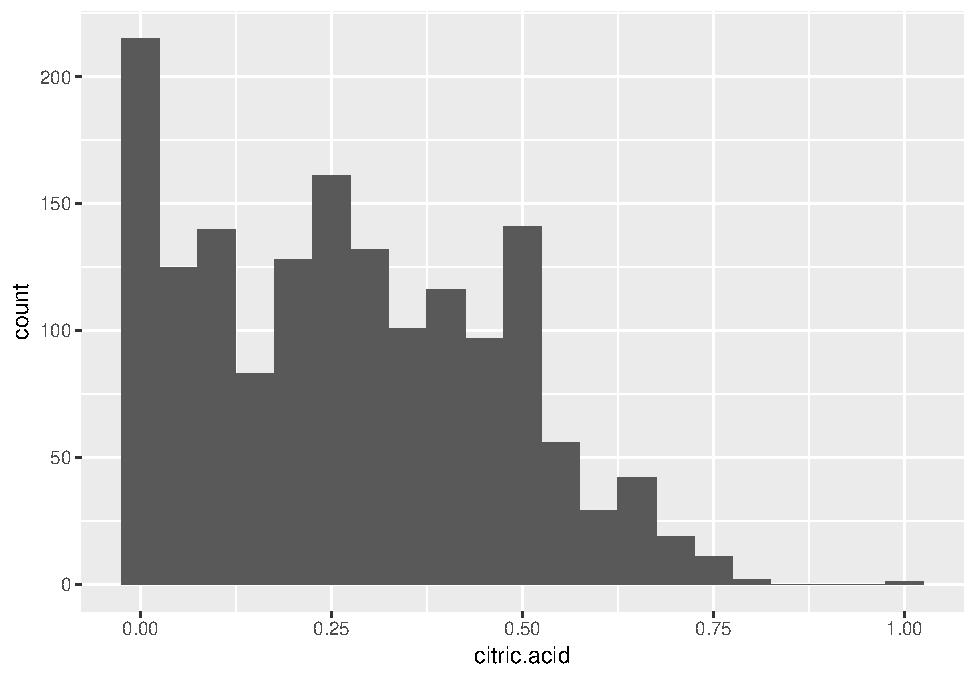
\includegraphics{RedWine_files/figure-latex/Make_Plot_Function_For_citric.acid-1.pdf}

The citric.acid also is skewed to the right.

\paragraph{Here is a summary about the citric.acid
variable.}\label{here-is-a-summary-about-the-citric.acid-variable.}

\begin{verbatim}
##    Min. 1st Qu.  Median    Mean 3rd Qu.    Max. 
##   0.000   0.090   0.260   0.271   0.420   1.000
\end{verbatim}

The above table shows a summary of the citric.acid variable.

\paragraph{Here is a histogram about the pH
variable.}\label{here-is-a-histogram-about-the-ph-variable.}

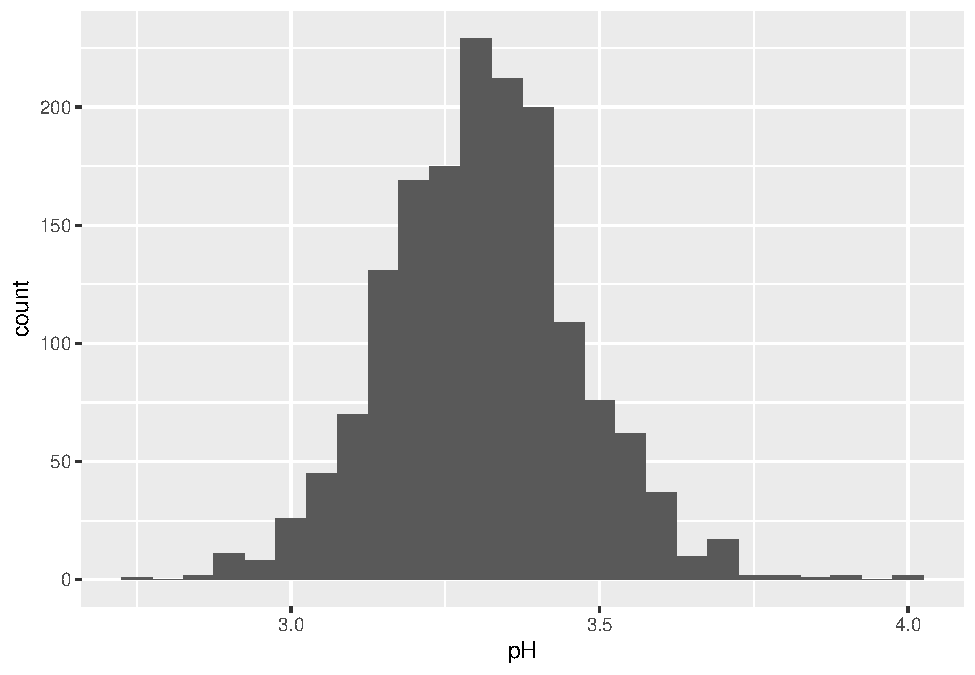
\includegraphics{RedWine_files/figure-latex/Make_Plot_Function_For_pH-1.pdf}

The pH is normally distributed.

\paragraph{Here is a summary about the pH
variable.}\label{here-is-a-summary-about-the-ph-variable.}

\begin{verbatim}
##    Min. 1st Qu.  Median    Mean 3rd Qu.    Max. 
##   2.740   3.210   3.310   3.311   3.400   4.010
\end{verbatim}

The above table shows a summary of the pH variable.

\paragraph{Here is a histogram about the chlorides
variable.}\label{here-is-a-histogram-about-the-chlorides-variable.}

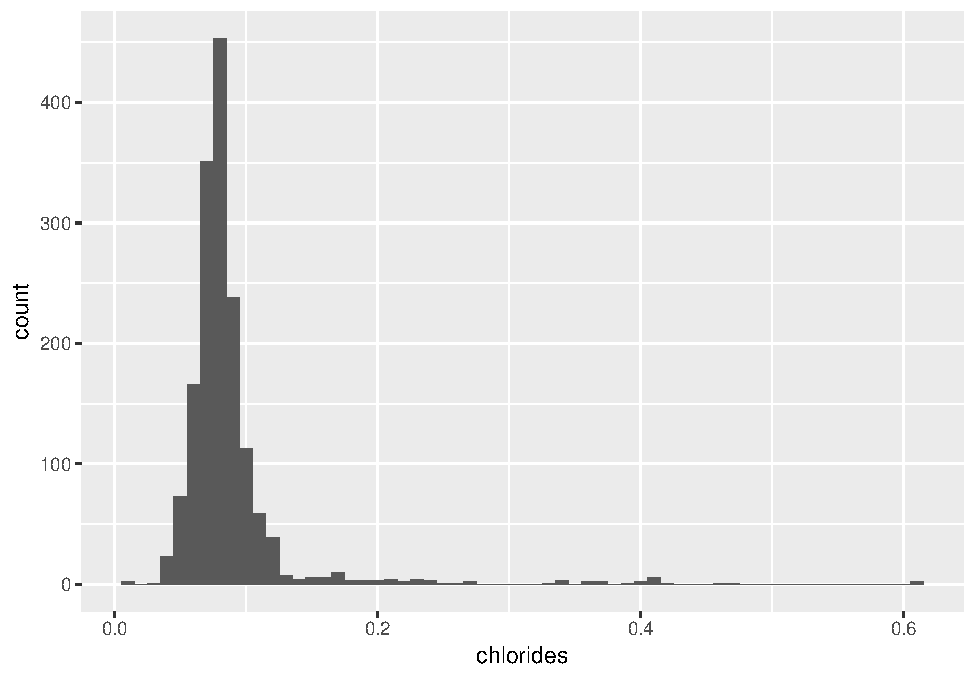
\includegraphics{RedWine_files/figure-latex/Make_Plot_Function_For_chlorides-1.pdf}

The chlorides is skewed to the right. \emph{We are going to apply the
10th log to it.}

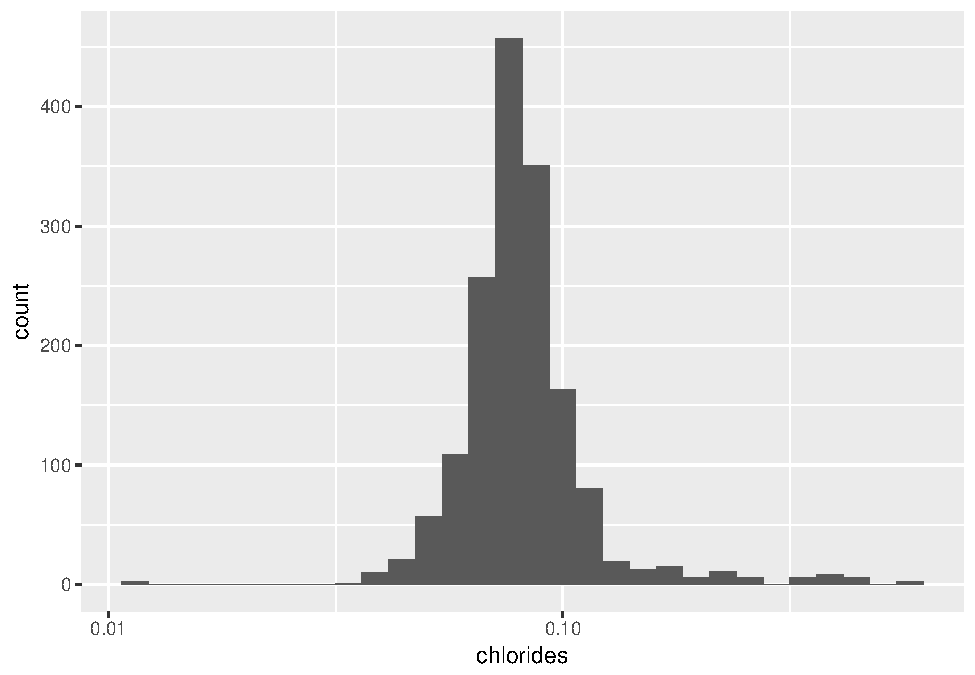
\includegraphics{RedWine_files/figure-latex/Make_Plot_Function_For_chlorides_log10-1.pdf}

The distribution of chlorides is normally distributed.

\paragraph{Here is a summary about the chlorides
variable.}\label{here-is-a-summary-about-the-chlorides-variable.}

\begin{verbatim}
##    Min. 1st Qu.  Median    Mean 3rd Qu.    Max. 
## 0.01200 0.07000 0.07900 0.08747 0.09000 0.61100
\end{verbatim}

The above table shows a summary of the chlorides variable.

\paragraph{Here is a histogram about the residual.sugar
variable.}\label{here-is-a-histogram-about-the-residual.sugar-variable.}

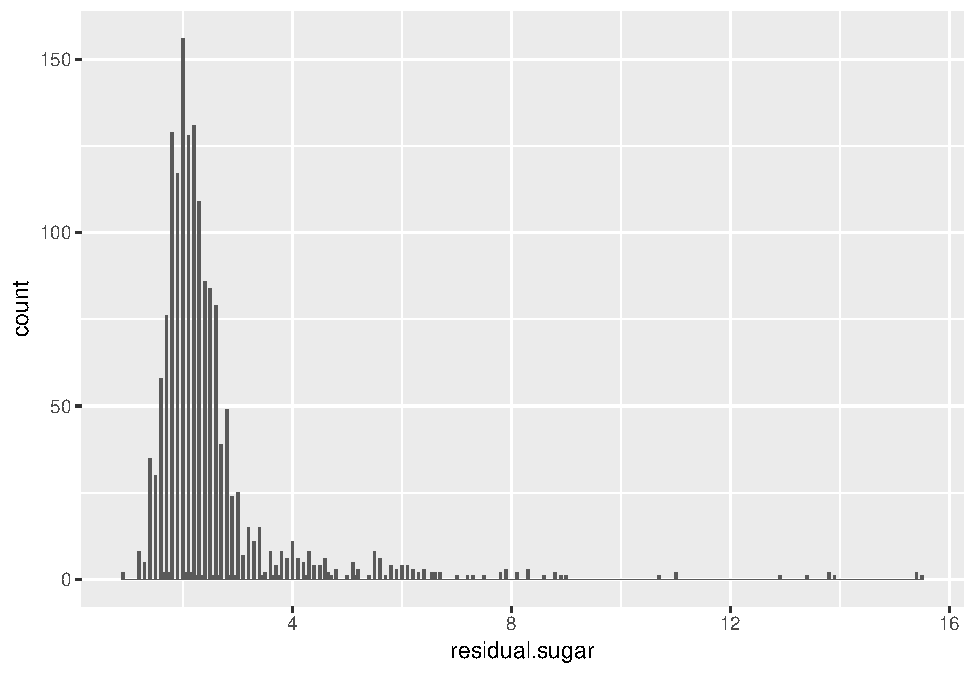
\includegraphics{RedWine_files/figure-latex/Make_Plot_Function_For_residual.sugar-1.pdf}

The residual.sugar is skewed to the right. \emph{We are going to apply
the 10th log to it.}

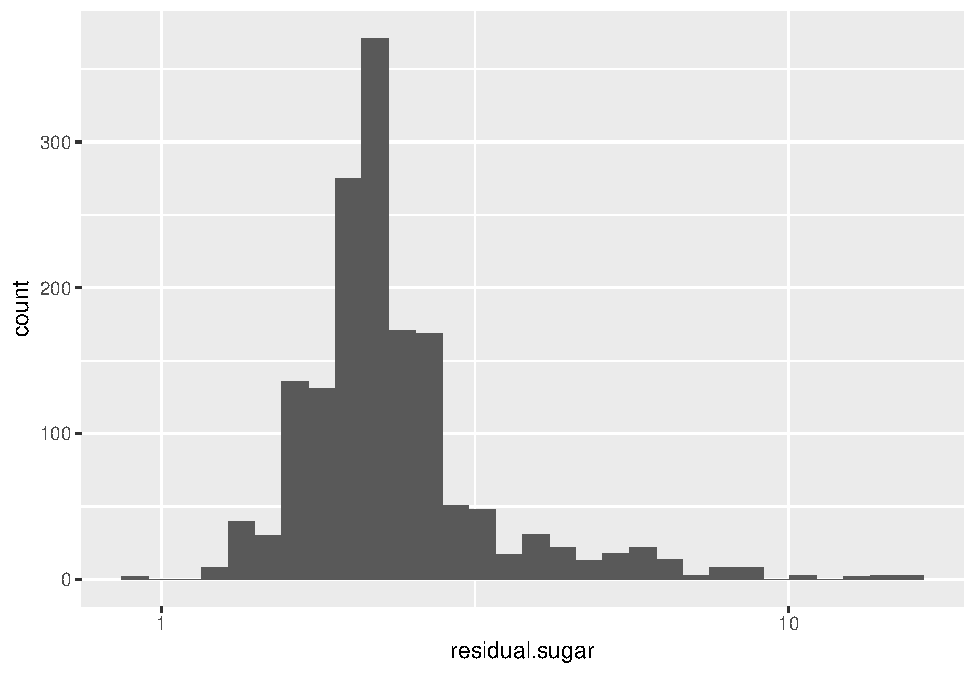
\includegraphics{RedWine_files/figure-latex/Make_Plot_Function_For_residual.sugar_log10-1.pdf}

The distribution of residual.sugar is normally distributed.

\paragraph{Here is a summary about the residual.sugar
variable.}\label{here-is-a-summary-about-the-residual.sugar-variable.}

\begin{verbatim}
##    Min. 1st Qu.  Median    Mean 3rd Qu.    Max. 
##   0.900   1.900   2.200   2.539   2.600  15.500
\end{verbatim}

The above table shows a summary of the residual.sugar variable.

\paragraph{Here is a histogram about the density
variable.}\label{here-is-a-histogram-about-the-density-variable.}

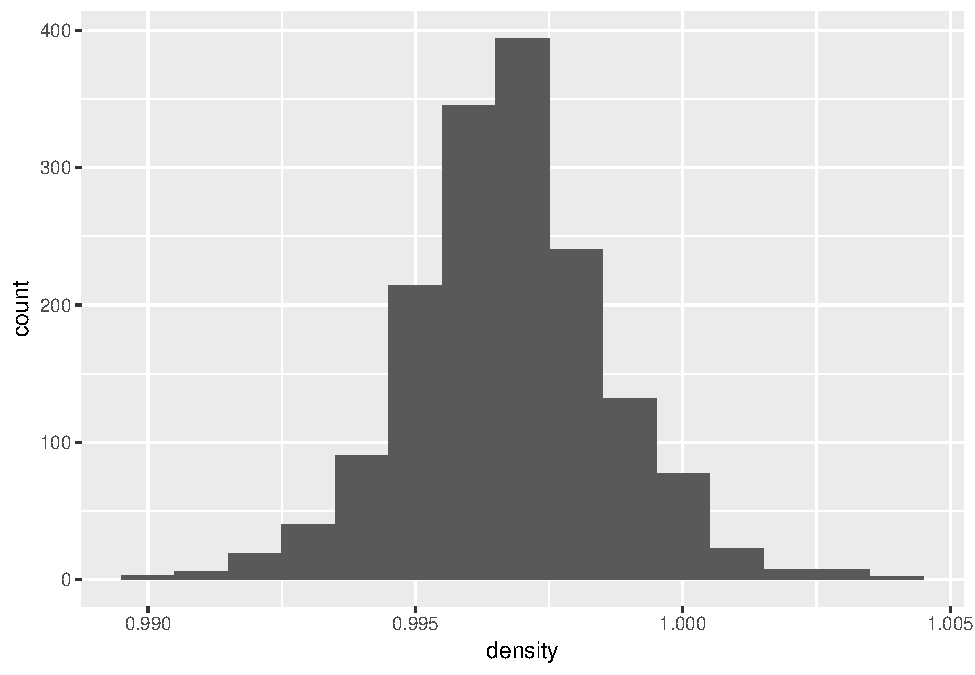
\includegraphics{RedWine_files/figure-latex/Make_Plot_Function_For_density-1.pdf}

The density is normally distributed.

\paragraph{Here is a summary about the density
variable.}\label{here-is-a-summary-about-the-density-variable.}

\begin{verbatim}
##    Min. 1st Qu.  Median    Mean 3rd Qu.    Max. 
##  0.9901  0.9956  0.9968  0.9967  0.9978  1.0037
\end{verbatim}

The above table shows a summary of the density variable.

\paragraph{Here is a histogram and box plot about the alcohol
variable.}\label{here-is-a-histogram-and-box-plot-about-the-alcohol-variable.}

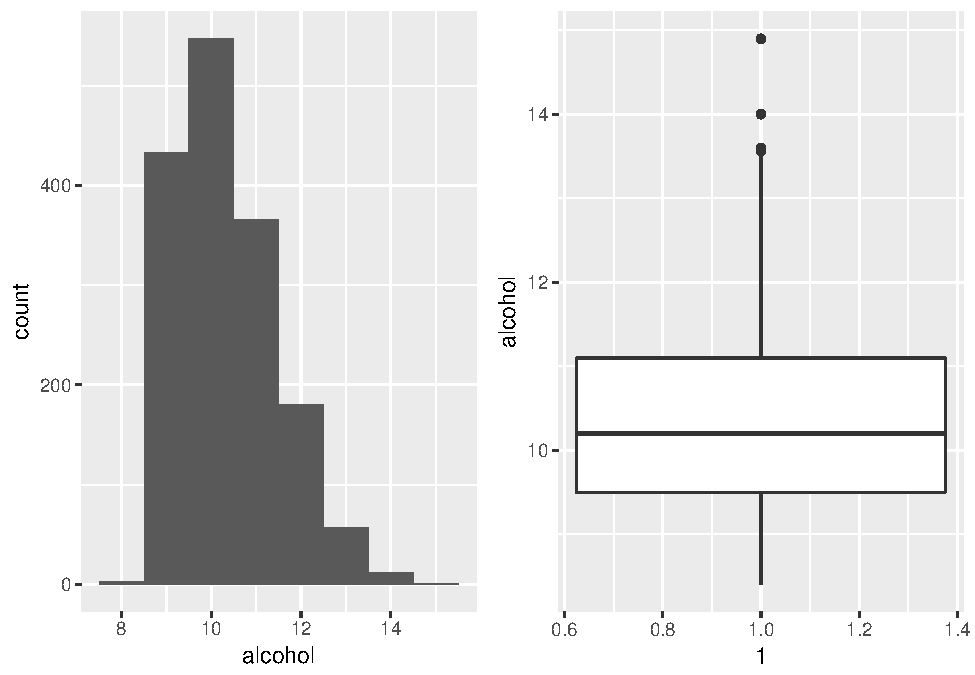
\includegraphics{RedWine_files/figure-latex/Make_Plot_For_alcohol-1.pdf}

We can see that most of alcohol exists from 9 to 11.

\paragraph{Here is a summary about the alcohol
variable.}\label{here-is-a-summary-about-the-alcohol-variable.}

\begin{verbatim}
##    Min. 1st Qu.  Median    Mean 3rd Qu.    Max. 
##    8.40    9.50   10.20   10.42   11.10   14.90
\end{verbatim}

The above table shows a summary of the alcohol variable.

\paragraph{Here is a histogram about the free.sulfur.dioxide
variable.}\label{here-is-a-histogram-about-the-free.sulfur.dioxide-variable.}

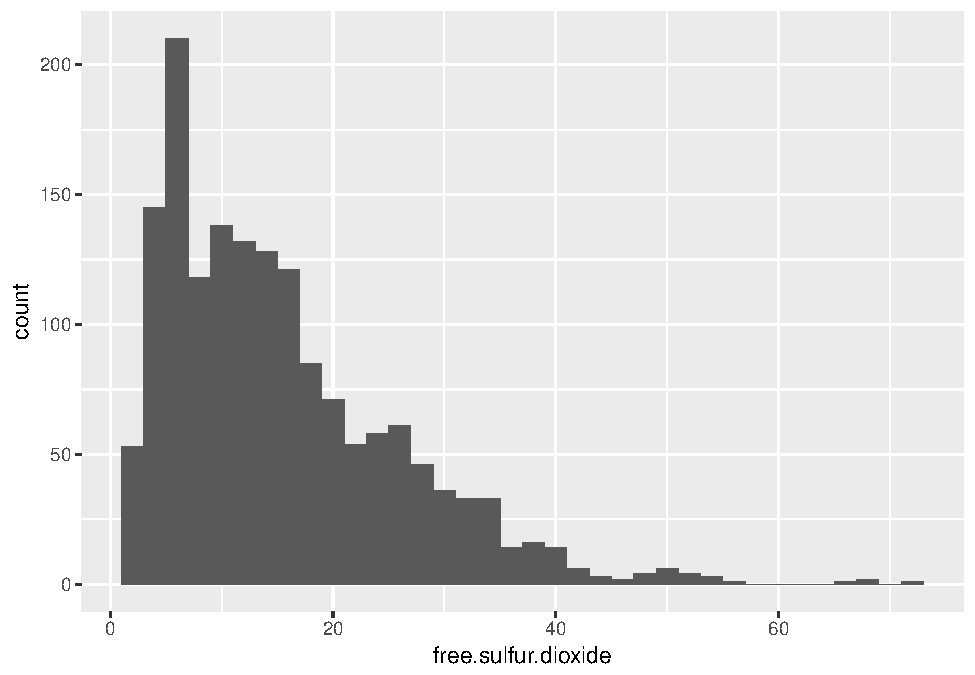
\includegraphics{RedWine_files/figure-latex/Make_Plot_Function_For_free.sulfur.dioxide-1.pdf}

The free.sulfur.dioxide is skewed to the right. \emph{We are going to
apply the 10th log to it.}

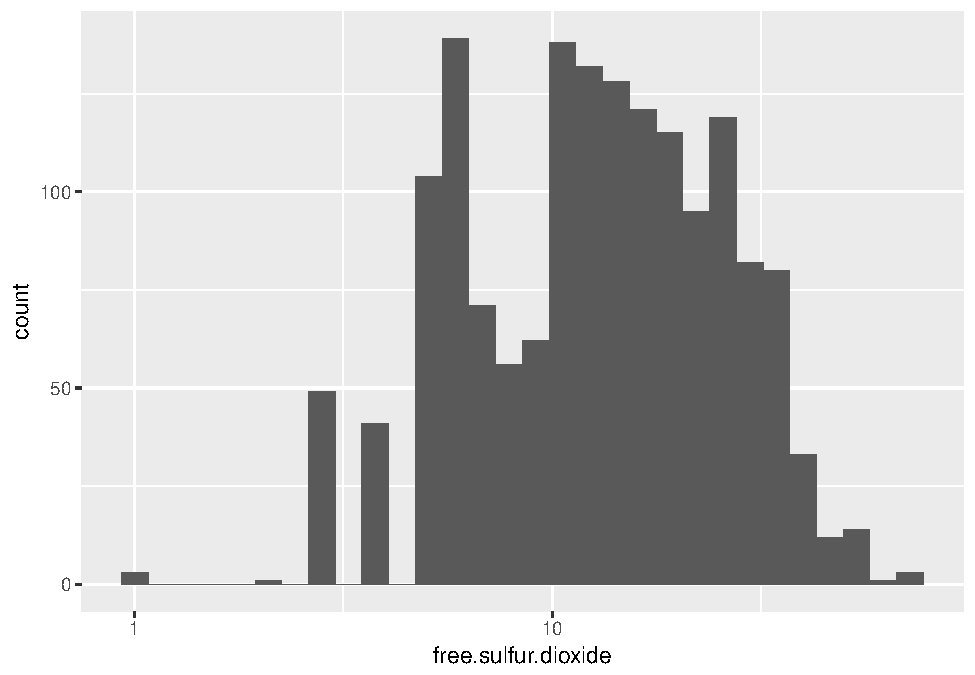
\includegraphics{RedWine_files/figure-latex/Make_Plot_Function_For_free.sulfur.dioxide_log10-1.pdf}

The distribution of free.sulfur.dioxide isn't normally distributed. It
seems to be like a bimodal distribution. Because free.sulfur.dioxide
near to 9 is very low.

\paragraph{Here is a summary about the free.sulfur.dioxide
variable.}\label{here-is-a-summary-about-the-free.sulfur.dioxide-variable.}

\begin{verbatim}
##    Min. 1st Qu.  Median    Mean 3rd Qu.    Max. 
##    1.00    7.00   14.00   15.87   21.00   72.00
\end{verbatim}

The above table shows a summary of the free.sulfur.dioxide variable.

\paragraph{Here is a histogram about the total.sulfur.dioxide
variable.}\label{here-is-a-histogram-about-the-total.sulfur.dioxide-variable.}

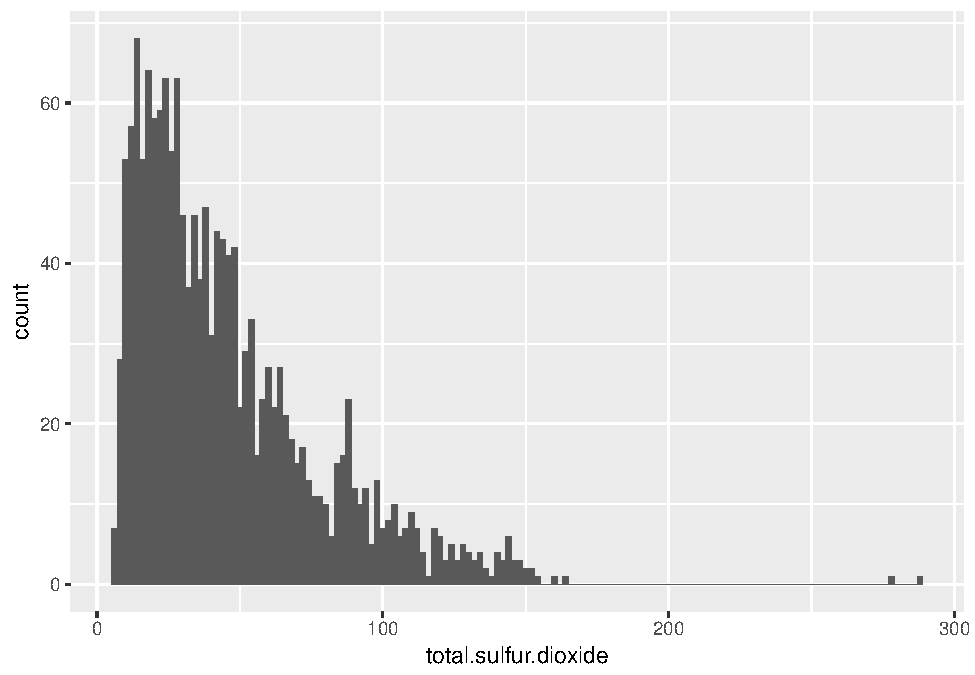
\includegraphics{RedWine_files/figure-latex/Make_Plot_Function_For_total.sulfur.dioxide-1.pdf}

The total.sulfur.dioxide is skewed to the right. \emph{We are going to
apply the 10th log to it.}

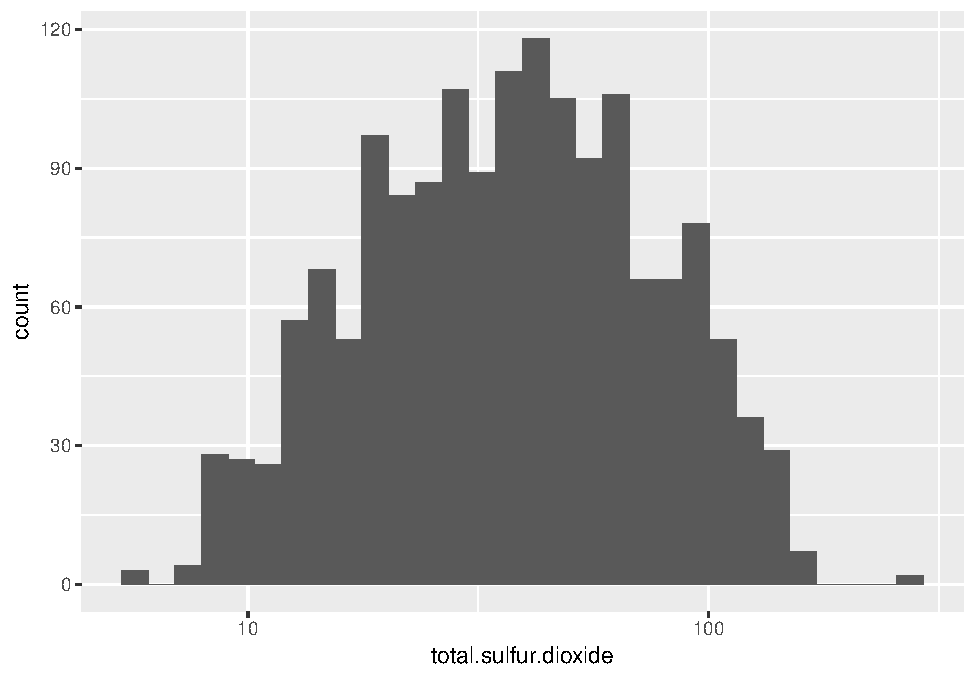
\includegraphics{RedWine_files/figure-latex/Make_Plot_Function_For_total.sulfur.dioxide_log10-1.pdf}

The distribution of total.sulfur.dioxide is normally distributed.

\paragraph{Here is a summary about the total.sulfur.dioxide
variable.}\label{here-is-a-summary-about-the-total.sulfur.dioxide-variable.}

\begin{verbatim}
##    Min. 1st Qu.  Median    Mean 3rd Qu.    Max. 
##    6.00   22.00   38.00   46.47   62.00  289.00
\end{verbatim}

The above table shows a summary of the total.sulfur.dioxide variable.

\paragraph{Here is a histogram about the volatile.acidity
variable.}\label{here-is-a-histogram-about-the-volatile.acidity-variable.}

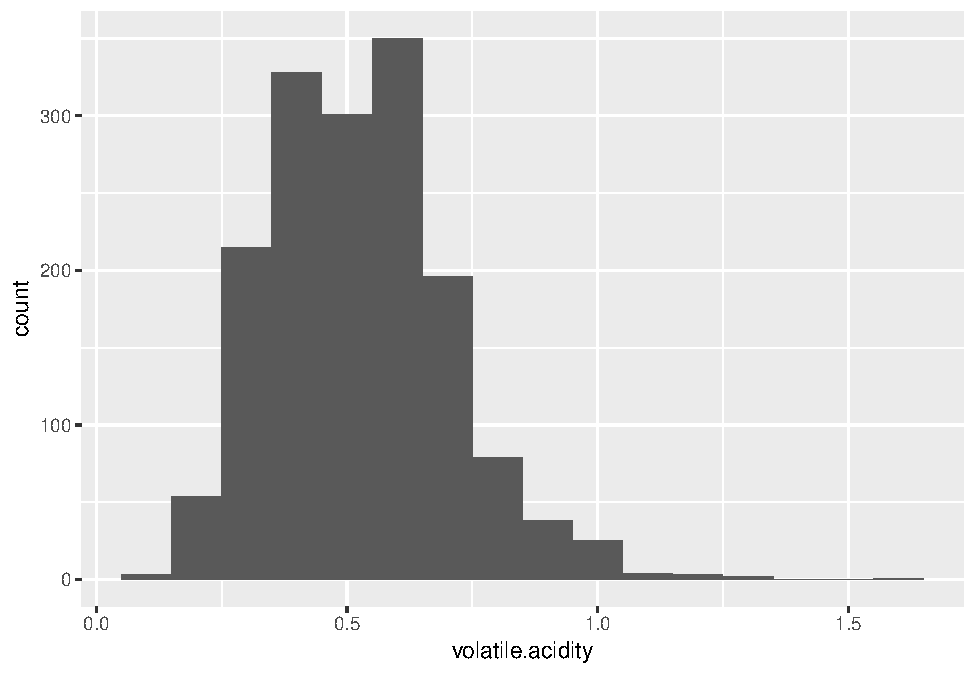
\includegraphics{RedWine_files/figure-latex/Make_Plot_Function_For_volatile.acidity-1.pdf}

The volatile.acidity is normally distributed.

\paragraph{Here is a summary about the volatile.acidity
variable.}\label{here-is-a-summary-about-the-volatile.acidity-variable.}

\begin{verbatim}
##    Min. 1st Qu.  Median    Mean 3rd Qu.    Max. 
##  0.1200  0.3900  0.5200  0.5278  0.6400  1.5800
\end{verbatim}

The above table shows a summary of the volatile.acidity variable.

\section{Univariate Analysis}\label{univariate-analysis}

\subsubsection{What is the structure of your
dataset?}\label{what-is-the-structure-of-your-dataset}

Red Wine dataset contains 1599 records. Also, it has 14 variables. And
this is the structure

\begin{verbatim}
##  [1] "fixed.acidity"        "volatile.acidity"     "citric.acid"         
##  [4] "residual.sugar"       "chlorides"            "free.sulfur.dioxide" 
##  [7] "total.sulfur.dioxide" "density"              "pH"                  
## [10] "sulphates"            "alcohol"              "quality"             
## [13] "category"             "ranking"
\end{verbatim}

\subsubsection{What is/are the main feature(s) of interest in your
dataset?}\label{what-isare-the-main-features-of-interest-in-your-dataset}

For sure, main interest is in quality variable. We are going to see how
it get affected by variables like percentage of alcohol, density and
chlorides.

\subsubsection{\texorpdfstring{What other features in the dataset do you
think will help support your\\
investigation into your feature(s) of
interest?}{What other features in the dataset do you think will help support your investigation into your feature(s) of interest?}}\label{what-other-features-in-the-dataset-do-you-think-will-help-support-your-investigation-into-your-features-of-interest}

Category and ranking will help me in the investigation into my features
of interest.

\subsubsection{Did you create any new variables from existing variables
in the
dataset?}\label{did-you-create-any-new-variables-from-existing-variables-in-the-dataset}

Yes, as listed above. I created the \emph{category} of wine {[}Light,
Medium, Strong{]} and \emph{rating} of wine {[}Poor, Good, Excellent{]}

\subsubsection{\texorpdfstring{Of the features you investigated, were
there any unusual distributions?\\
Did you perform any operations on the data to tidy, adjust, or change
the form\\
of the data? If so, why did you do
this?}{Of the features you investigated, were there any unusual distributions? Did you perform any operations on the data to tidy, adjust, or change the form of the data? If so, why did you do this?}}\label{of-the-features-you-investigated-were-there-any-unusual-distributions-did-you-perform-any-operations-on-the-data-to-tidy-adjust-or-change-the-form-of-the-data-if-so-why-did-you-do-this}

Some variabels like {[}residual.sugar \& alcohol{]} are skewed to the
right. So, I made a log10 transformation to them to be normally
distributed. I did because they always affect the quality.

\section{Bivariate Plots Section}\label{bivariate-plots-section}

We are going to group our sample based on the quality of it. We will
have the mean volatile.acidity and median volatile.acidity also the
number of occurence.

\begin{verbatim}
## # A tibble: 6 × 4
##   quality mean_volatile.acidity median_volatile.acidity     n
##     <int>                 <dbl>                   <dbl> <int>
## 1       3             0.8845000                   0.845    10
## 2       4             0.6939623                   0.670    53
## 3       5             0.5770411                   0.580   681
## 4       6             0.4974843                   0.490   638
## 5       7             0.4039196                   0.370   199
## 6       8             0.4233333                   0.370    18
\end{verbatim}

And here is a summary about the new variable rw.quality

\begin{verbatim}
##     quality     mean_volatile.acidity median_volatile.acidity
##  Min.   :3.00   Min.   :0.4039        Min.   :0.3700         
##  1st Qu.:4.25   1st Qu.:0.4419        1st Qu.:0.4000         
##  Median :5.50   Median :0.5373        Median :0.5350         
##  Mean   :5.50   Mean   :0.5800        Mean   :0.5542         
##  3rd Qu.:6.75   3rd Qu.:0.6647        3rd Qu.:0.6475         
##  Max.   :8.00   Max.   :0.8845        Max.   :0.8450         
##        n         
##  Min.   : 10.00  
##  1st Qu.: 26.75  
##  Median :126.00  
##  Mean   :266.50  
##  3rd Qu.:528.25  
##  Max.   :681.00
\end{verbatim}

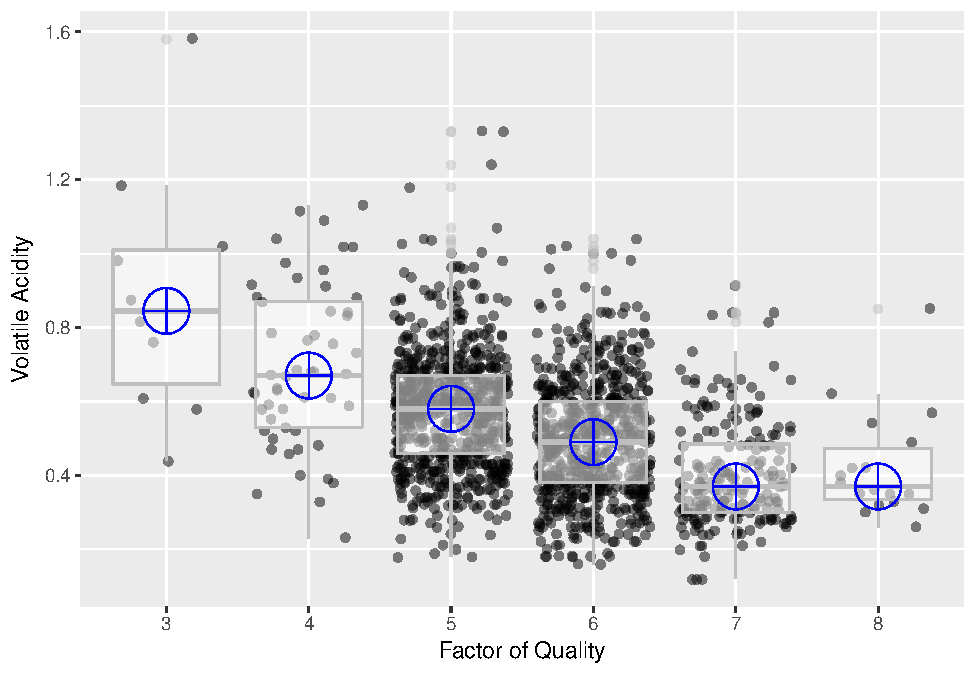
\includegraphics{RedWine_files/figure-latex/Quality_Vs_Volatile.Acidity-1.pdf}

Our dataset contains some outlier, so we used median. We can see that as
the quality increses, the volatile acidity decreases.

\begin{verbatim}
##                      fixed.acidity volatile.acidity citric.acid
## fixed.acidity                1.000           -0.256       0.672
## volatile.acidity            -0.256            1.000      -0.552
## citric.acid                  0.672           -0.552       1.000
## residual.sugar               0.115            0.002       0.144
## chlorides                    0.094            0.061       0.204
## free.sulfur.dioxide         -0.154           -0.011      -0.061
## total.sulfur.dioxide        -0.113            0.076       0.036
## density                      0.668            0.022       0.365
## pH                          -0.683            0.235      -0.542
## sulphates                    0.183           -0.261       0.313
## alcohol                     -0.062           -0.202       0.110
## quality                      0.124           -0.391       0.226
##                      residual.sugar chlorides free.sulfur.dioxide
## fixed.acidity                 0.115     0.094              -0.154
## volatile.acidity              0.002     0.061              -0.011
## citric.acid                   0.144     0.204              -0.061
## residual.sugar                1.000     0.056               0.187
## chlorides                     0.056     1.000               0.006
## free.sulfur.dioxide           0.187     0.006               1.000
## total.sulfur.dioxide          0.203     0.047               0.668
## density                       0.355     0.201              -0.022
## pH                           -0.086    -0.265               0.070
## sulphates                     0.006     0.371               0.052
## alcohol                       0.042    -0.221              -0.069
## quality                       0.014    -0.129              -0.051
##                      total.sulfur.dioxide density     pH sulphates alcohol
## fixed.acidity                      -0.113   0.668 -0.683     0.183  -0.062
## volatile.acidity                    0.076   0.022  0.235    -0.261  -0.202
## citric.acid                         0.036   0.365 -0.542     0.313   0.110
## residual.sugar                      0.203   0.355 -0.086     0.006   0.042
## chlorides                           0.047   0.201 -0.265     0.371  -0.221
## free.sulfur.dioxide                 0.668  -0.022  0.070     0.052  -0.069
## total.sulfur.dioxide                1.000   0.071 -0.066     0.043  -0.206
## density                             0.071   1.000 -0.342     0.149  -0.496
## pH                                 -0.066  -0.342  1.000    -0.197   0.206
## sulphates                           0.043   0.149 -0.197     1.000   0.094
## alcohol                            -0.206  -0.496  0.206     0.094   1.000
## quality                            -0.185  -0.175 -0.058     0.251   0.476
##                      quality
## fixed.acidity          0.124
## volatile.acidity      -0.391
## citric.acid            0.226
## residual.sugar         0.014
## chlorides             -0.129
## free.sulfur.dioxide   -0.051
## total.sulfur.dioxide  -0.185
## density               -0.175
## pH                    -0.058
## sulphates              0.251
## alcohol                0.476
## quality                1.000
\end{verbatim}

We can see that there is a highe correlation between alcohol and
quality.

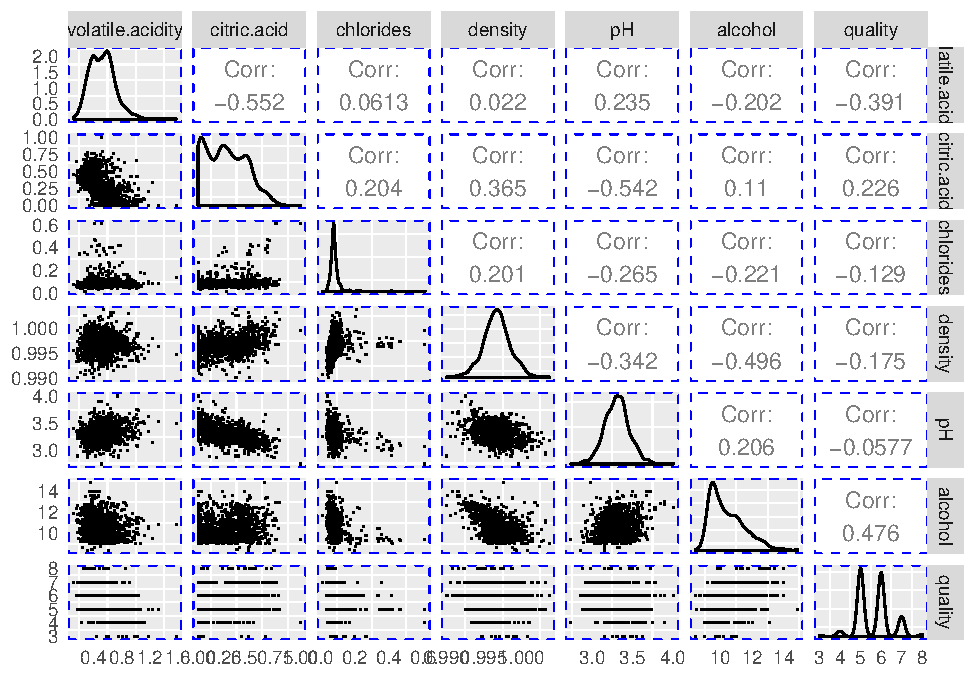
\includegraphics{RedWine_files/figure-latex/Correlations_Diagram-1.pdf}

The above visualization shows a strong correlation between quality \&
alcohol. Also, it shows negtibe correlation between volatile.acidity \&
quality and cetric.acid \& pH.

\emph{Now, we will check relation between pH and alcohol.}

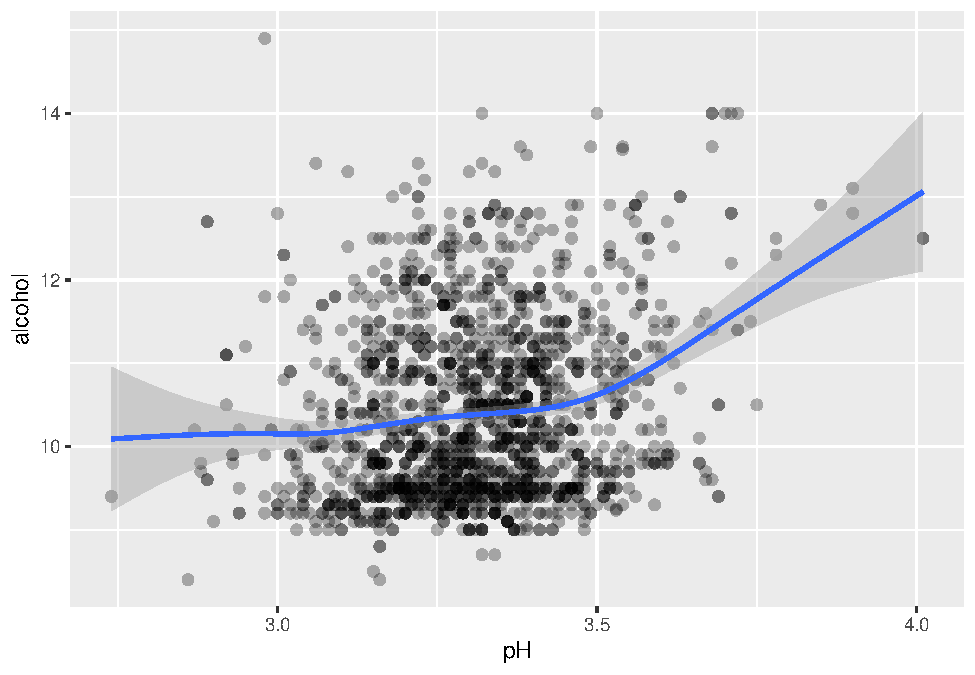
\includegraphics{RedWine_files/figure-latex/Correlation_Diagram-1.pdf}

\emph{The above visualization shows low correlation, so we are going to
check it with correlation test}

\begin{verbatim}
## 
##  Pearson's product-moment correlation
## 
## data:  rw$pH and rw$alcohol
## t = 8.397, df = 1597, p-value < 2.2e-16
## alternative hypothesis: true correlation is not equal to 0
## 95 percent confidence interval:
##  0.1582061 0.2521123
## sample estimates:
##       cor 
## 0.2056325
\end{verbatim}

As expected, now much correlation between them.

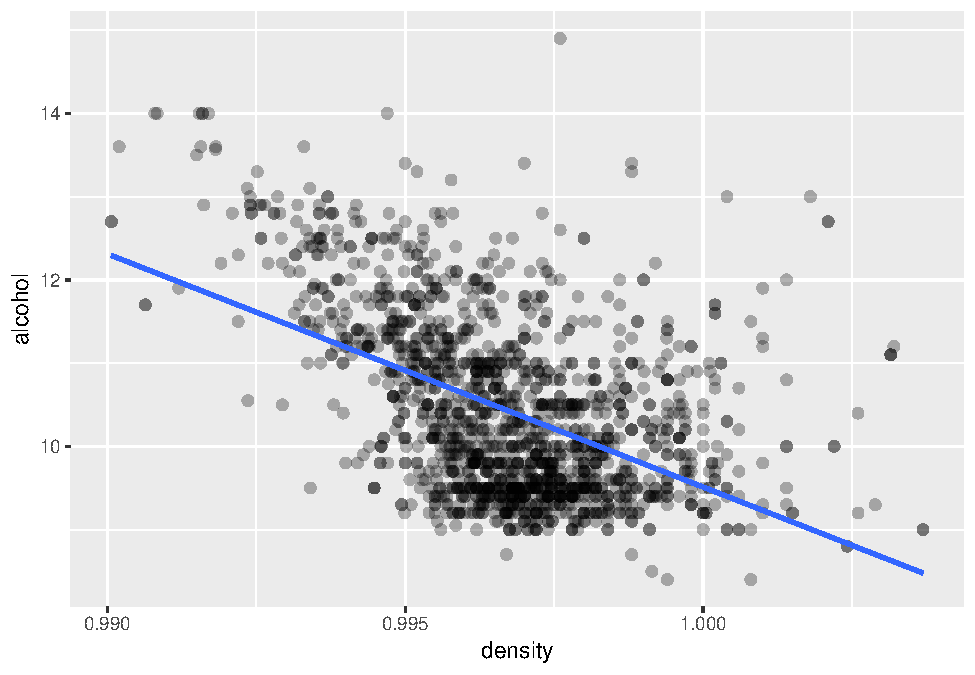
\includegraphics{RedWine_files/figure-latex/density_And_alcohol-1.pdf}

\emph{The above visualization shows some correlation, so we are going to
check it with correlation test}

\begin{verbatim}
## 
##  Pearson's product-moment correlation
## 
## data:  rw$density and rw$alcohol
## t = -22.838, df = 1597, p-value < 2.2e-16
## alternative hypothesis: true correlation is not equal to 0
## 95 percent confidence interval:
##  -0.5322547 -0.4583061
## sample estimates:
##        cor 
## -0.4961798
\end{verbatim}

We can see that there is a negtive correlation between {[}density,
alcohol{]}.

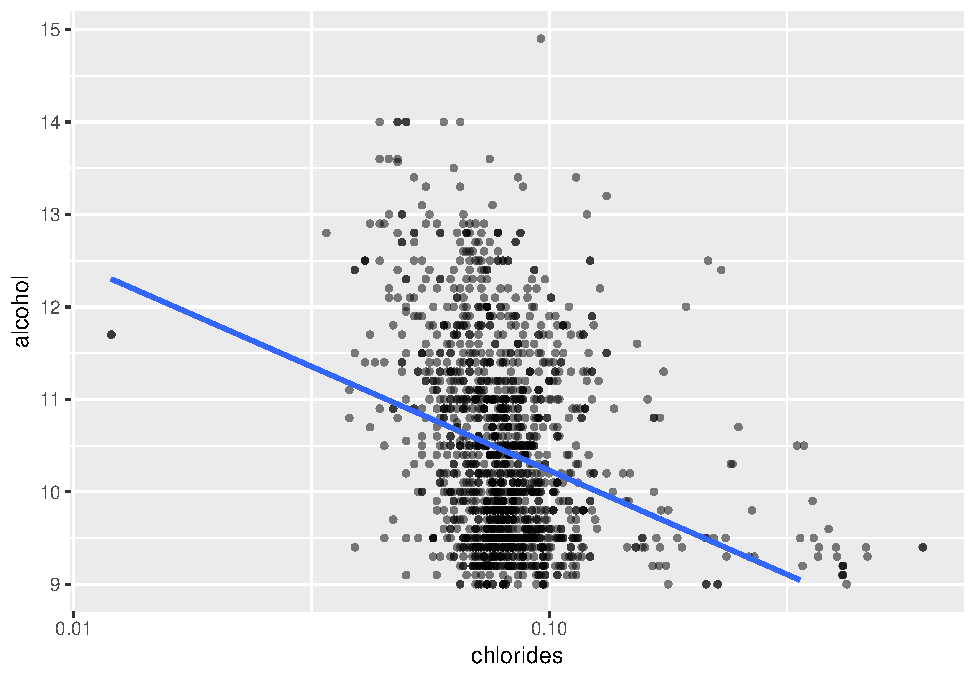
\includegraphics{RedWine_files/figure-latex/chlorides_And_alcohol-1.pdf}

\emph{The above visualization shows outlaier, so we are going to check
it with correlation test}

\begin{verbatim}
## 
##  Pearson's product-moment correlation
## 
## data:  rw$chlorides and rw$alcohol
## t = -9.0617, df = 1597, p-value < 2.2e-16
## alternative hypothesis: true correlation is not equal to 0
## 95 percent confidence interval:
##  -0.2672644 -0.1740057
## sample estimates:
##        cor 
## -0.2211405
\end{verbatim}

We can see that there is no much correlation between {[}chlorides,
alcohol{]}.

\section{Bivariate Analysis}\label{bivariate-analysis}

\subsubsection{\texorpdfstring{Talk about some of the relationships you
observed in this part of the\\
investigation. How did the feature(s) of interest vary with other
features in\\
the
dataset?}{Talk about some of the relationships you observed in this part of the investigation. How did the feature(s) of interest vary with other features in the dataset?}}\label{talk-about-some-of-the-relationships-you-observed-in-this-part-of-the-investigation.-how-did-the-features-of-interest-vary-with-other-features-in-the-dataset}

\begin{enumerate}
\def\labelenumi{\arabic{enumi}.}
\tightlist
\item
  Density with alcohol: When alcohol increases, density decreases.
\item
  Residual sugar with alcohol: weak.
\item
  Acidic with pH: weak.
\end{enumerate}

\subsubsection{\texorpdfstring{Did you observe any interesting
relationships between the other features\\
(not the main feature(s) of
interest)?}{Did you observe any interesting relationships between the other features (not the main feature(s) of interest)?}}\label{did-you-observe-any-interesting-relationships-between-the-other-features-not-the-main-features-of-interest}

The relationship between alcohol \& density, When alcohol increases,
density decreases.

\subsubsection{What was the strongest relationship you
found?}\label{what-was-the-strongest-relationship-you-found}

I was expecting many strong relationships, but the dataset shows
nothing.

\section{Multivariate Plots Section}\label{multivariate-plots-section}

\begin{quote}
\textbf{Tip}: Now it's time to put everything together. Based on what
you found in the bivariate plots section, create a few multivariate
plots to investigate more complex interactions between variables. Make
sure that the plots that you create here are justified by the plots you
explored in the previous section. If you plan on creating any
mathematical models, this is the section where you will do that.
\end{quote}

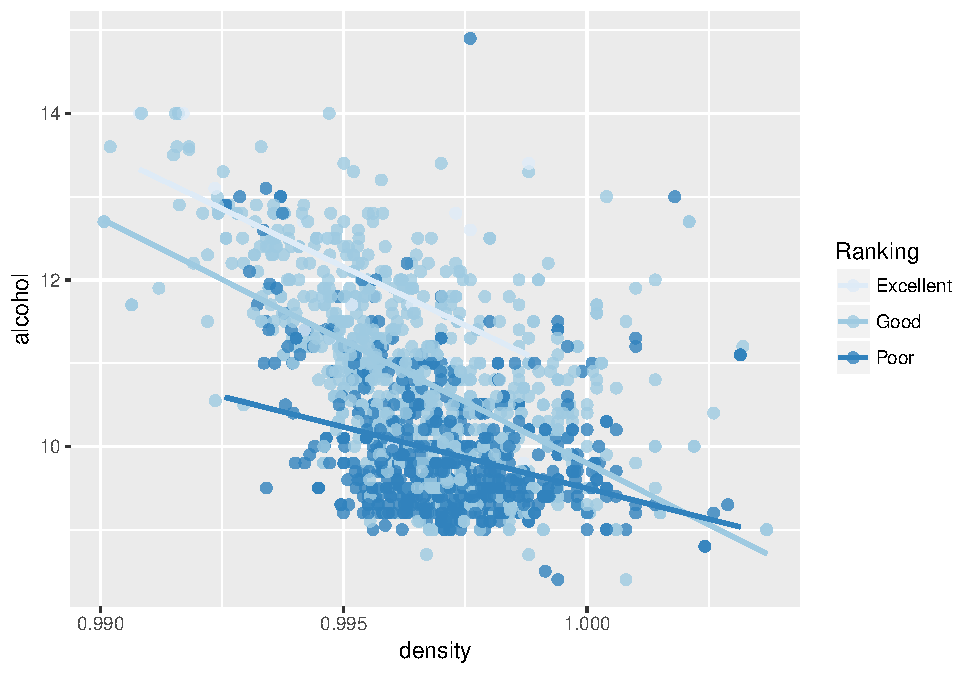
\includegraphics{RedWine_files/figure-latex/Multivariate_Plots-1.pdf}

\includegraphics{RedWine_files/figure-latex/Multivariate_Plots_pH\&Alcohol-1.pdf}

The above two visualizations show that the excellent wine has a higer
alcohol.

\section{Multivariate Analysis}\label{multivariate-analysis}

\subsubsection{\texorpdfstring{Talk about some of the relationships you
observed in this part of the\\
investigation. Were there features that strengthened each other in terms
of\\
looking at your feature(s) of
interest?}{Talk about some of the relationships you observed in this part of the investigation. Were there features that strengthened each other in terms of looking at your feature(s) of interest?}}\label{talk-about-some-of-the-relationships-you-observed-in-this-part-of-the-investigation.-were-there-features-that-strengthened-each-other-in-terms-of-looking-at-your-features-of-interest}

I can clrearly see that alcohol and density affact the ranking of the
wine.

\subsubsection{Were there any interesting or surprising interactions
between
features?}\label{were-there-any-interesting-or-surprising-interactions-between-features}

Ranking with other variables.

\begin{center}\rule{0.5\linewidth}{\linethickness}\end{center}

\section{Final Plots and Summary}\label{final-plots-and-summary}

\subsubsection{Plot One}\label{plot-one}

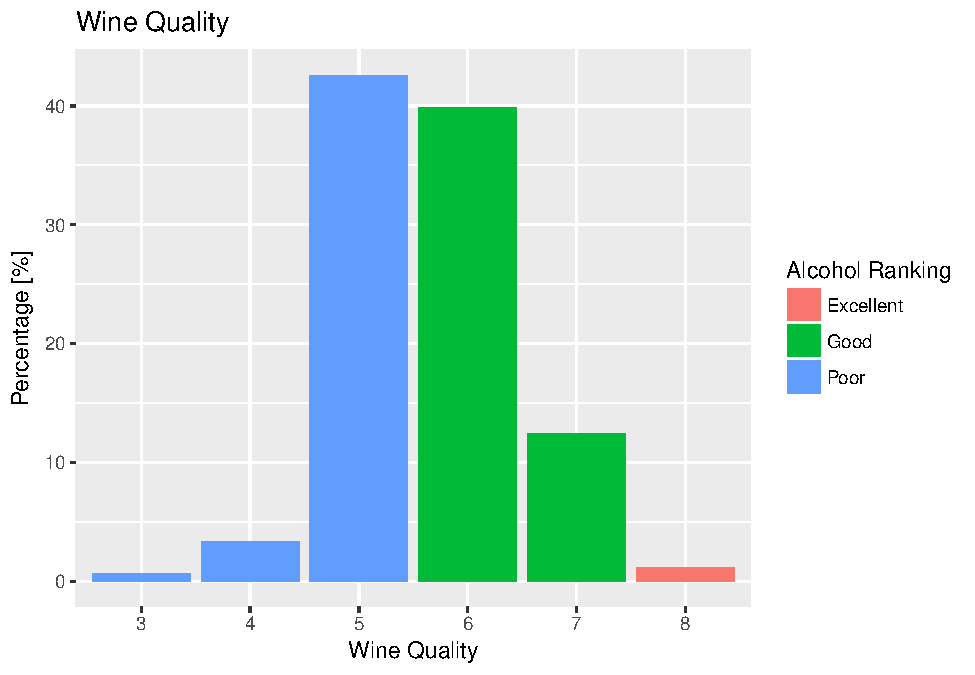
\includegraphics{RedWine_files/figure-latex/Plot_One-1.pdf}

\subsubsection{Description One}\label{description-one}

visualization shows that most of the sample quality are between {[}5,
6{]}. Excellent wines are with higher alcohol, more than 7. And poor are
lower than 6. So, to select better wine, try to find one with alcohol
\textgreater{}= 7.

\subsubsection{Plot Two}\label{plot-two}

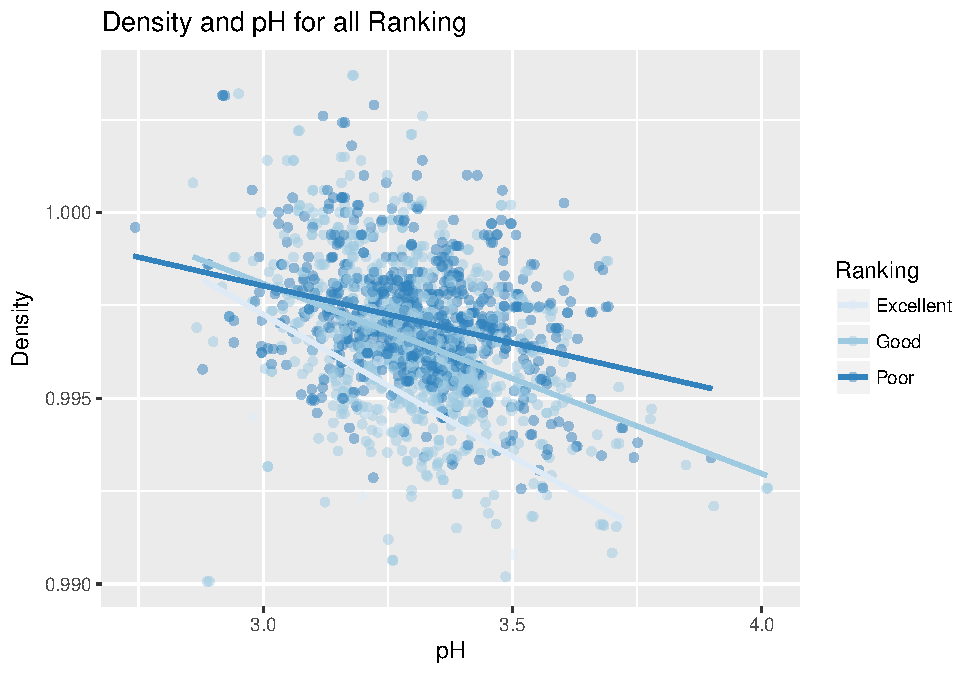
\includegraphics{RedWine_files/figure-latex/Plot_Two-1.pdf}

\subsubsection{Description Two}\label{description-two}

The above visualization shows that as the density increases, the pH
decreases. Which means there is a negative correlation. Excellent red
wines have pH between {[}3.0, 3.5{]} and the density lower than 1.0.

\subsubsection{Plot Three}\label{plot-three}

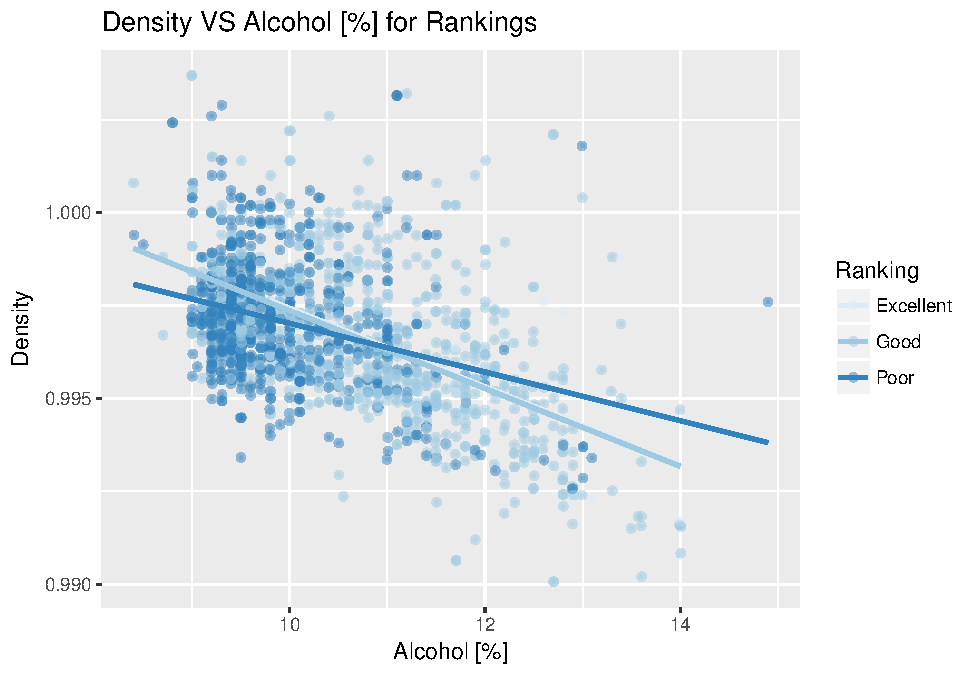
\includegraphics{RedWine_files/figure-latex/Plot_Three-1.pdf}

\subsubsection{Description Three}\label{description-three}

We can see that there is a strong correlation between alcohol \&
density. As alcohol increase, density decrease. This means better wines
are with high alcohol and low Density. And poor wines are with high
density and low alcohol.

\begin{center}\rule{0.5\linewidth}{\linethickness}\end{center}

\section{Reflection}\label{reflection}

For me, I had no experience in wines because I don't drink them. Also, I
didn't expect that wines have massive characteristics. But when I
started investigating the dataset, I learned a lot about wines world and
how they get ranked and categorized. This is a very interesting topic
because they have a huge fan. I took a longer time in the investigation
to read about the chemicals and how they linked together, it was really
fun.

After understanding the dataset, I started the analysis. It was my first
experiment with R Language, so I faced some problems at the beginning.

The dataset was really well organized, but I added two variables
{[}Ranking and Category{]} to help me in my analysis. We can see that
alcohol \& density are the best indicators of the wine quality. This
will help all people who drink red wine to take better decisions based
on chemical details.

For the feature, I am planning to get a bigger dataset to increase the
sample size and get a better understanding of this area. Also, I think I
am going to make a small mobile app, where you take a picture for your
selection of wine, then the app will make some analysis about it.


\end{document}
